\begin{frame}[allowframebreaks]
  \frametitle{A New Perspective}
  $$S:y^2 = 2s^4 + 8ms^2 + 16m^2 + 16m$$
  \phantom{hi}
  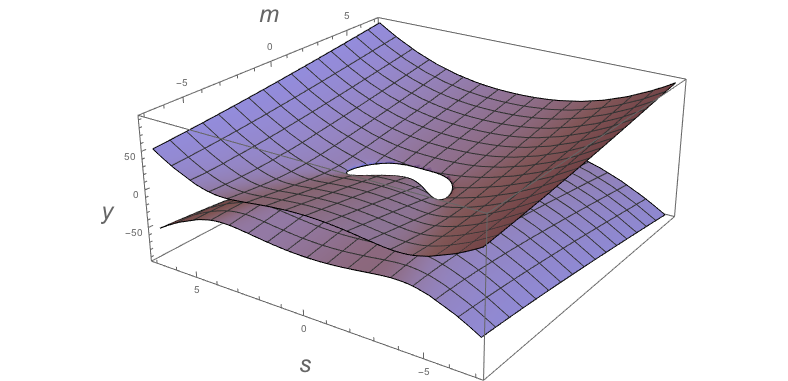
\includegraphics[width=\textwidth]{SPlot.png}
  
\framebreak
  
  So far,
	$$S:y^2 = 2s^4 + 8ms^2 + 16m^2 + 16m$$
	\phantom{hi}
	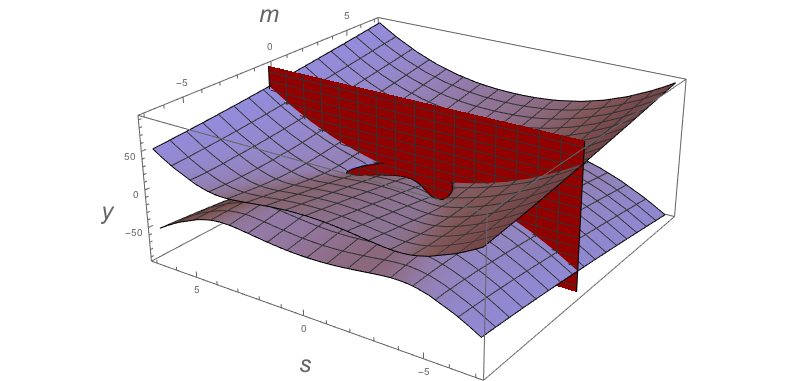
\includegraphics[width=\textwidth]{ECPlot.png}

\framebreak

	$$S:y^2 = 16m^2 + (16+8s^2)m + 2s^4$$
	\phantom{hi}
	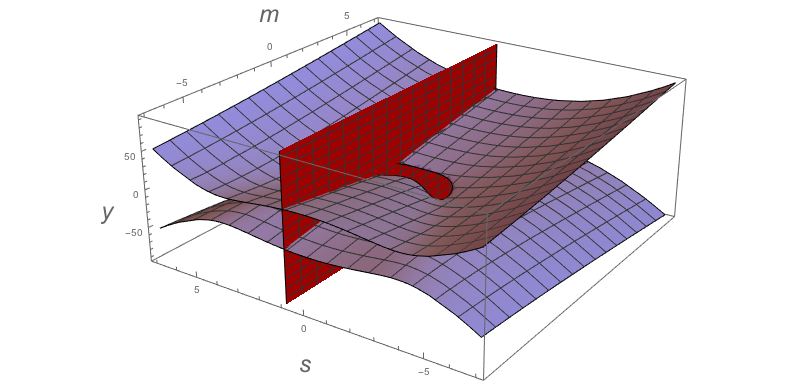
\includegraphics[width=\textwidth]{CSPlot.png}
	
	\framebreak
	
	This is a conic! $$y^2 = am^2 + bm + c$$
	\phantom{hi}
	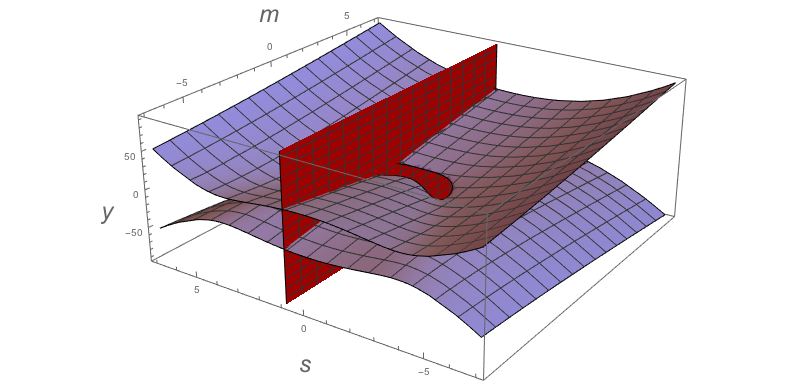
\includegraphics[width=\textwidth]{CSPlot.png}
\end{frame}

\begin{frame}
	\frametitle{Rational Projection}
	For any $s$, we have
	$$y^2 = 16m^2 + (16+8s^2)m + 2s^4.$$
	\pause
	\begin{center}
	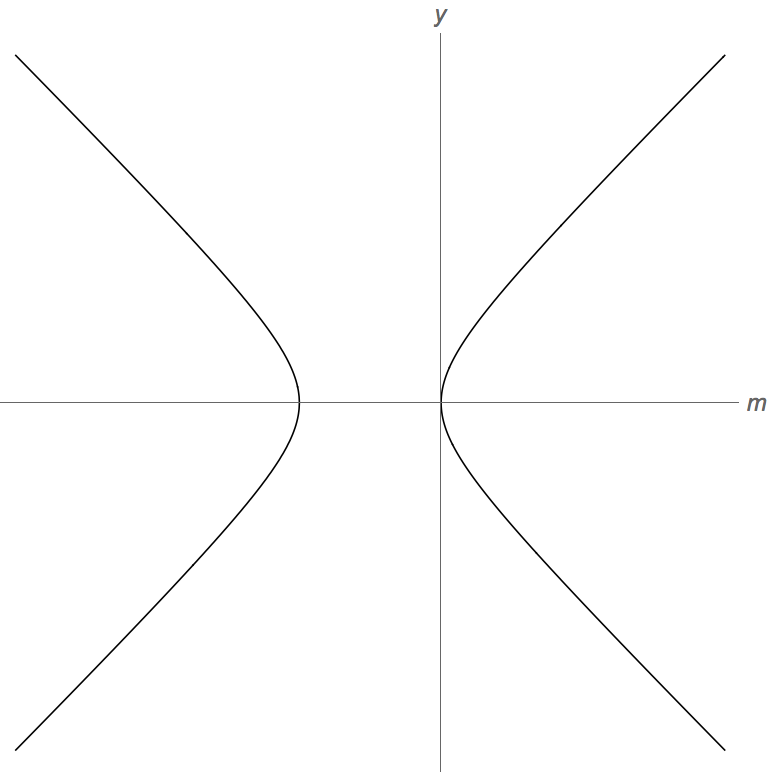
\includegraphics[width=0.5\textwidth]{s0Plot.png} \\
	Example: $s=0$
	\end{center}
\end{frame}
	
\begin{frame}
	\frametitle{Rational Projection}
	$$S: y^2 = 16m^2 + (16+8s^2)m + 2s^4$$
	\pause
	\begin{obs}
		We're only looking for \textbf{rational} solutions.
	\end{obs}
	\pause
	$$\mbox{Let }y = \frac{Y}{Z}\mbox{ and }m = \frac{M}{Z}.$$
	\pause
	\begin{defn}
		The \textbf{homogeneous form} of $S$ is
		$$S: Y^2 = 16 M^2 + (8 s^2 + 16) M Z + 2 s^4 Z^2.$$
	\end{defn}
\end{frame}

\begin{frame}
	\frametitle{Rational Projection}
	If $Z=0$...
	\pause
	$$Y^2 = 16 M^2 + (8 s^2 + 16) M Z + 2 s^4 Z^2$$
	\pause
	$$Y^2 = 16 M^2 +\text{ \hcancel{\ensuremath{(8 s^2 + 16) M Z}}} + \text{ \hcancel{\ensuremath{2 s^4 Z^2}}}$$
	\pause
	$$ Y^2 = 16 M^2 $$
	\pause
	$$ Y=\pm 4 M$$
	\pause
	\begin{obs}
	The point $[M:Y:Z]=[1:4:0]$ is a solution to the homogeneous form of $S$.
	\end{obs}
\end{frame}

\begin{frame}
	\frametitle{Rational Projection}
	Geometrically, this is a line with slope $4$.
	\begin{center}
		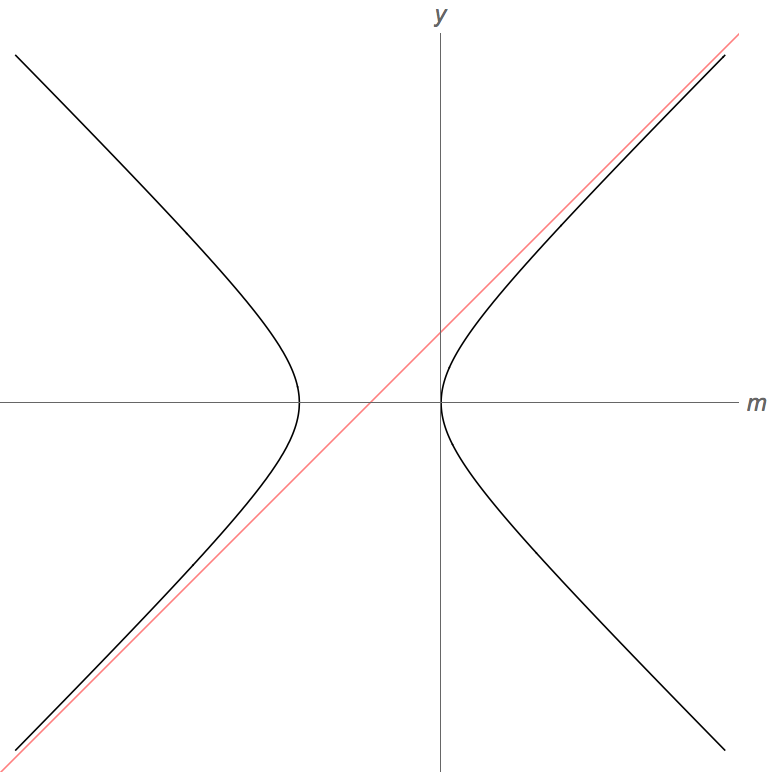
\includegraphics[width=.6\textwidth]{s0AsymptotePlot.png} \\
		Example: $s=0$ and $y=4m+2$
	\end{center}
\end{frame}

\begin{frame}
	\frametitle{Rational Projection}
	To project from the point at infinity, take any line with slope 4.
	\begin{center}
		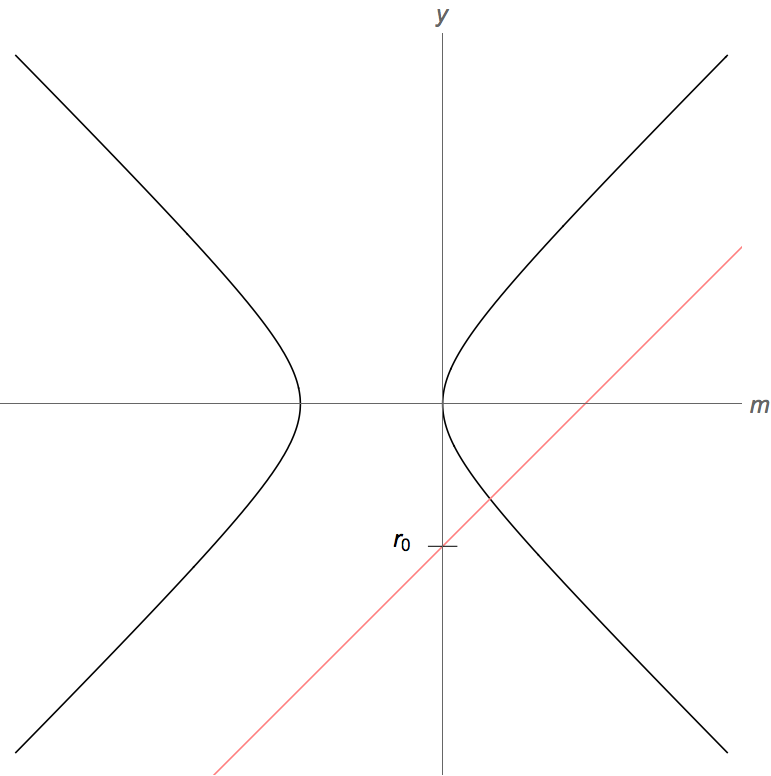
\includegraphics[width=.6\textwidth]{s0ProjectionPlot.png} \\
		Example: $s=0$ and $y=4m+r_0$
	\end{center}
\end{frame}

\begin{frame}
	\frametitle{Rational Projection}
	This intersects $S$ at a rational point:
	\begin{center}
		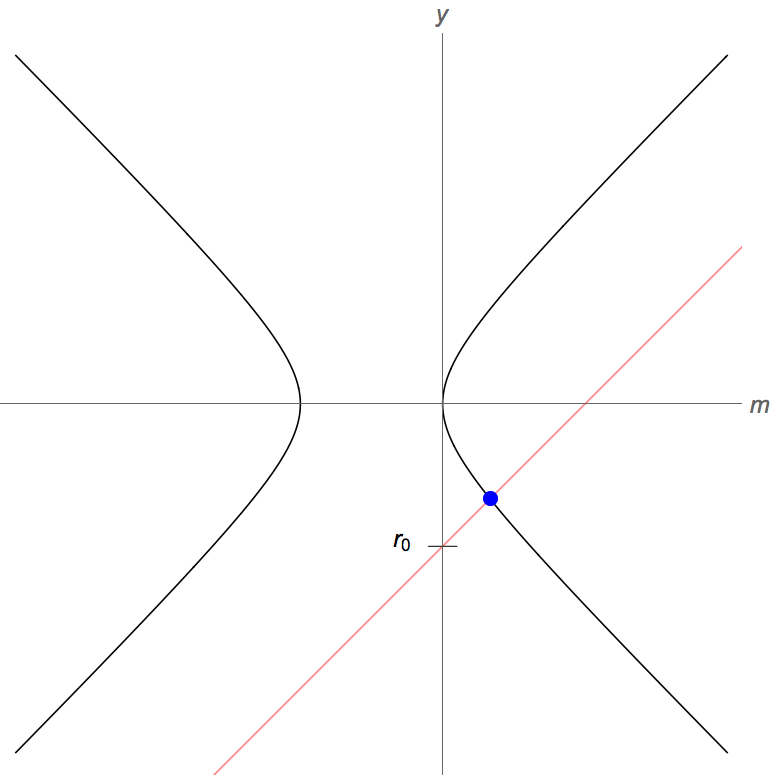
\includegraphics[width=.6\textwidth]{s0ProjectionIntersectionPlot.png} \\
		Example: $s=0$ and $y=4m+r_0$
	\end{center}
\end{frame}

\begin{frame}
	\frametitle{Rational Projection}
	Solving for this intersection point gives
	\begin{align*}
		m &= \frac{2 s^4-r_0^2}{8 r} \\
		\mbox{and }y &= \frac{-4 + r^2 - 4 s^2 + s^4}{2 r}
	\end{align*}
	$\mbox{where }r=\left(r_0-s^2-2\right).$\\
	\pause
	So for every rational $r$ and $s$, we get rational $m$ and $y$ such that
	$$ y^2 = 16m^2 + (16+8s^2)m + 2s^4 $$
\end{frame}

\begin{frame}
	\frametitle{Rational Projection}
	\begin{defn}
		We define this projection as $$ \phi(r,s) = (m(r,s),y(r,s)) $$ where $$m(r,s)=\frac{-4 - 4 r - r^2 - 4 s^2 - 2 r s^2 + s^4}{8r},$$ $$y(r,s)=\frac{-4 + r^2 - 4 s^2 + s^4}{2 r}  $$
	\end{defn}
\end{frame}

\begin{frame}
	\frametitle{Rational Projection}
	This gives us a value for $m$. Defining $f$ requires $m$ and $\gamma$. Luckily, we've already seen an equation for $\gamma$.
	\pause
	\begin{defn}
		\begin{align*}
			\begin{split}
				\gamma(r,s) = \pm\beta \left(- \frac{3 s^{6}}{16} - \frac{s^{4} m}{2} - \frac{s^{2} m^{2}}{2} - \frac{s^{2} m}{2}\right) + \frac{17 s^{8}}{64} + \frac{5 m}{4} s^{6} + \\ \frac{11 s^{4}}{4} m^{2} + \frac{7 m}{4} s^{4} + 2 s^{2} m^{3} + 2 s^{2} m^{2} - m
			\end{split}
		\end{align*}
	where $m=m(r,s)$ is given by our projection.
	\end{defn}
\end{frame}

\begin{frame}
	\frametitle{Rational Projection}
	\begin{example}
		If $r=1$ and $s=1$,
		$$\phi(r,s) = (m(r,s),y(r,s)) = \left(-\frac{7}{4},3\right)$$
		and
		$$\gamma(r,s) = \frac{1}{2}.$$
		\pause
		This gives the polynomial
		\begin{align*}
			f(x) &= \left(x-\frac{1}{2}\right)^2+\frac{1}{2}-\frac{7}{4} \\
			&= x^2 - x - 1.
		\end{align*}
		\pause
		This is the polynomial for the golden ratio!
	\end{example}
	
\end{frame}

\begin{frame}
	\frametitle{Rational Projection}
	\begin{itemize}
		\item<1-> Every newly reducible $f^3$ gives a point on $S$. \\
		\item<2-> So by choosing all $(r,s)$, we get all newly reducible $f^3$. \\
		\item<3-> However, we will also get some that are not \textbf{newly} reducible. \\
		\item<4-> How can we ensure that we get a newly reducible $f^3$?
	\end{itemize}
\end{frame}

\begin{frame}
	\frametitle{Finding Newly Reducible Third Iterates}
	Recall that
	\begin{align*}
		f\mbox{ is reducible } &\Leftrightarrow -m-\gamma\mbox{ is a square,} \\
		\mbox{and }f^2\mbox{ is newly reducible }&\Leftrightarrow2(-m\pm\sqrt{m^2+m+\gamma})\mbox{ is a square.}
	\end{align*}
	So if we have a point on $S$ and neither $-m-\gamma$ nor $m^2+m+\gamma$ is a square, $f^3$ is newly reducible.
\end{frame}

\begin{frame}
	\frametitle{Finding Newly Reducible Third Iterates}
	\begin{align*}
		\begin{split}
			-m-\gamma &=  \frac{1}{256 r^2} s^2 \left(r^2-2 (r+2) s^2+s^4-4\right)^2\left(4 + 2 r - s^2\right)
		\end{split}\\
		\begin{split}
			\begin{tabular}{r}$m^2+m+\gamma$ \\ \vphantom{x} \\ \vphantom{x} \end{tabular} & \begin{tabular}{l}$=$\\ \vphantom{x} \\ \vphantom{x} \end{tabular} \begin{tabular}{r} $\dfrac{1}{256 r^2}\left(r-s^2+2\right)^2 (16 + 16 r + 4 r^2 + 32 s^2 + 32 r s^2$ \\ $ + 4 r^2 s^2 - 2 r^3 s^2 + 8 s^4 + 12 r s^4 $ \\ $ + 5 r^2 s^4 - 8 s^6 - 4 r s^6 + s^8).$ \end{tabular}
		\end{split}
	\end{align*}
\end{frame}

\begin{frame}
	\frametitle{Finding Newly Reducible Third Iterates}
	\begin{align*}
		\begin{split}
			\left(4 + 2 r - s^2\right) \\
			\phantom{x} \\
			(16 + 16 r + 4 r^2 + 32 s^2 + 32 r s^2 + 4 r^2 s^2 - 2 r^3 s^2 + 8 s^4 + 12 r s^4 \\ + 5 r^2 s^4 - 8 s^6 - 4 r s^6 + s^8)
		\end{split}
	\end{align*}
\end{frame}

\begin{frame}
	\frametitle{Finding Newly Reducible Third Iterates}
	\begin{align*}
		\begin{split}
		\left(4 + 2 r - s^2\right) \\
		\phantom{x} \\
		(16 + 16 r + 4 r^2 + 32 s^2 + 32 r s^2 + 4 r^2 s^2 \hunder{$- 2 r^3 s^2$} + 8 s^4 + 12 r s^4 \\ + 5 r^2 s^4 - 8 s^6 - 4 r s^6 + s^8)
		\end{split}
	\end{align*}
	\pause
	Let $r$ be "big enough"
\end{frame}






















